\documentclass[12pt]{article}
\usepackage[T1]{fontenc}
\usepackage[utf8]{inputenc}
\usepackage{amsmath}
\usepackage[left=2cm,right=2cm,top=1cm,bottom=2cm]{geometry}
\usepackage{enumitem}
\usepackage{tikz}
\usepackage{multicol}

\pagestyle{empty}

\newcommand{\answerbox}{\tikz \draw (0,0) rectangle ++(0.3cm,0.3cm);}
\newcommand{\filledbox}{\tikz \fill[black] (0,0) rectangle ++(0.3cm,0.3cm);}
\newcommand{\numbox}{\tikz \draw (0,0) rectangle ++(0.15cm,0.15cm);}
\newcommand{\correctedbox}{
    
\begin{tikzpicture}
        \fill[black] (0,0) rectangle ++(0.3cm,0.3cm);
        \draw[red, line width=0.8pt] (0.15cm,0.15cm) circle[radius=0.25cm];
    \end{tikzpicture}
}


\begin{document}

\begin{center}
\textbf{\Huge Antwortblatt} \\
\vspace{0.3cm}
\textbf{Prüfung aus Quantitative Methoden 2, 2.5.24} \\
\vspace{0.3cm}
%\textbf{\large 20. Dezember 2023}
\end{center}
\vspace{0.5cm}

\begin{tabular}{@{}p{0.5\textwidth}p{0.5\textwidth}@{}}
  Name: & Matrikelnummer: \\
  \vspace{5mm} & \vspace{5mm} \\
\end{tabular}

\vspace{10mm}

\noindent Identifikationsnummer:

\bigskip

\noindent
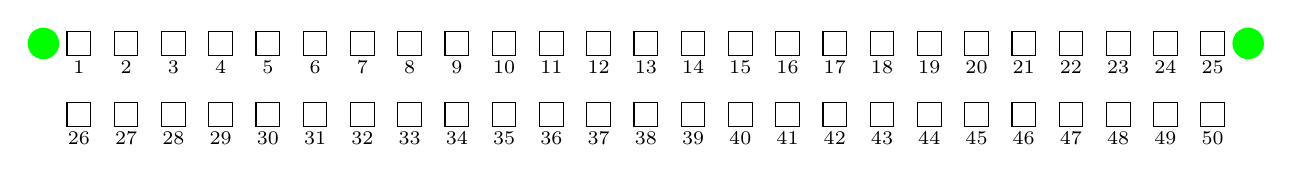
\begin{tikzpicture}[x=0.6cm, y=0.6cm] % Raster beibehalten

% Grüner Punkt links neben der ersten Nummer
  \fill[green] (0.5, 0.25) circle (0.2cm);

  % Erste Zeile mit 25 Kästchen
  \foreach \x in {1,...,25} {
    \draw (\x, 0) rectangle +(0.5, 0.5); % Größe der Boxen beibehalten
    \node at (\x+0.25, -0.25) {\scriptsize \x}; % Position der Nummerierung beibehalten
  }
  
  % Grüner Punkt rechts neben der 25. Nummer
  \fill[green] (26, 0.25) circle (0.2cm);
  
  % Zweite Zeile mit 25 Kästchen, Abstand erhöht
  \foreach \x in {26,...,50} {
    \draw ({(\x-25)}, -1.5) rectangle +(0.5, 0.5); % Vertikaler Abstand auf 1.5 erhöht
    \node at ({(\x-25)+0.25}, -1.75) {\scriptsize \x}; % Position der Nummerierung angepasst
  }
\end{tikzpicture}
\vspace{5mm}

\noindent \textbf{Anweisungen:} Bitte färben Sie die richtigen Antworten in den dafür vorgesehenen Kästchen mit einem schwarzen Filzstift ein. Nur die hier angekreuzten Antworten werden gewertet.\\
Anleitung, wie angekreuzt (ausgemalt) wird - \textbf{Korrekturen} dürfen \textbf{nur auf dem} extra \textbf{Korrekturenblatt} durchgeführt werden:

        \begin{tabular}{cccc}
            A) \filledbox & B) \answerbox & C) \filledbox & D) \answerbox
        \end{tabular}


\vspace{0.5cm}

% Fügen Sie dies am Anfang des Fragebereichs hinzu
\begin{tikzpicture}[remember picture, overlay]
  % Angepasste Positionen für die Ankerpunkte
  % Oben links
  \node at (current page.north west) [shift={(2cm,-12.8cm)}] {
    \begin{tikzpicture}
      \fill[red] (0,0) circle (0.2cm);
      %\draw (0,-0.2) -- (0,0.2);
      %\draw (-0.2,0) -- (0.2,0);
    \end{tikzpicture}
  };
  % Oben rechts
  \node at (current page.north east) [shift={(-3.8cm,-12.8cm)}] {
    
\begin{tikzpicture}
      \fill[red] (0,0) circle (0.2cm);
      %\draw (0,-0.2) -- (0,0.2);
      %\draw (-0.2,0) -- (0.2,0);
    \end{tikzpicture}
  };
  % Unten links
  \node at (current page.south west) [shift={(2cm,2.3cm)}] {
    
\begin{tikzpicture}
      \fill[red] (0,0) circle (0.2cm);
      %\draw (0,-0.2) -- (0,0.2);
      %\draw (-0.2,0) -- (0.2,0);
    \end{tikzpicture}
  };
  % Unten rechts
  \node at (current page.south east) [shift={(-3.8cm,2.3cm)}] {
    
\begin{tikzpicture}
      \fill[red] (0,0) circle (0.2cm);
      %\draw (0,-0.2) -- (0,0.2);
      %\draw (-0.2,0) -- (0.2,0);
    \end{tikzpicture}
  };
\end{tikzpicture}



\begin{multicols}{2}
\begin{enumerate}[itemsep=0.3cm]
    \item
        \begin{tabular}{cccc}
            A) \answerbox & B) \answerbox & C) \answerbox & D) \answerbox
        \end{tabular}
    
    \item
        \begin{tabular}{cccc}
            A) \answerbox & B) \answerbox & C) \answerbox & D) \answerbox
        \end{tabular}

    \item
        \begin{tabular}{cccc}
            A) \answerbox & B) \answerbox & C) \answerbox & D) \answerbox
        \end{tabular}

    \item
        \begin{tabular}{cccc}
            A) \answerbox & B) \answerbox & C) \answerbox & D) \answerbox
        \end{tabular}

    \item
        \begin{tabular}{cccc}
            A) \answerbox & B) \answerbox & C) \answerbox & D) \answerbox
        \end{tabular}

    \item
        \begin{tabular}{cccc}
            A) \answerbox & B) \answerbox & C) \answerbox & D) \answerbox
        \end{tabular}
   
    \item
        \begin{tabular}{cccc}
            A) \answerbox & B) \answerbox & C) \answerbox & D) \answerbox
        \end{tabular}

    \item
        \begin{tabular}{cccc}
            A) \answerbox & B) \answerbox & C) \answerbox & D) \answerbox
        \end{tabular}

    \item
        \begin{tabular}{cccc}
            A) \answerbox & B) \answerbox & C) \answerbox & D) \answerbox
        \end{tabular}

    \item
        \begin{tabular}{cccc}
            A) \answerbox & B) \answerbox & C) \answerbox & D) \answerbox
        \end{tabular}

\item
        \begin{tabular}{cccc}
            A) \answerbox & B) \answerbox & C) \answerbox & D) \answerbox
        \end{tabular}
    
    \item
        \begin{tabular}{cccc}
            A) \answerbox & B) \answerbox & C) \answerbox & D) \answerbox
        \end{tabular}

    \item
        \begin{tabular}{cccc}
            A) \answerbox & B) \answerbox & C) \answerbox & D) \answerbox
        \end{tabular}

    \item
        \begin{tabular}{cccc}
            A) \answerbox & B) \answerbox & C) \answerbox & D) \answerbox
        \end{tabular}

    \item
        \begin{tabular}{cccc}
            A) \answerbox & B) \answerbox & C) \answerbox & D) \answerbox
        \end{tabular}

    \item
        \begin{tabular}{cccc}
            A) \answerbox & B) \answerbox & C) \answerbox & D) \answerbox
        \end{tabular}
   
    \item
        \begin{tabular}{cccc}
            A) \answerbox & B) \answerbox & C) \answerbox & D) \answerbox
        \end{tabular}

    \item
        \begin{tabular}{cccc}
            A) \answerbox & B) \answerbox & C) \answerbox & D) \answerbox
        \end{tabular}

    \item
        \begin{tabular}{cccc}
            A) \answerbox & B) \answerbox & C) \answerbox & D) \answerbox
        \end{tabular}

    \item
        \begin{tabular}{cccc}
            A) \answerbox & B) \answerbox & C) \answerbox & D) \answerbox
        \end{tabular}

\item
        \begin{tabular}{cccc}
            A) \answerbox & B) \answerbox & C) \answerbox & D) \answerbox
        \end{tabular}
   
    \item
        \begin{tabular}{cccc}
            A) \answerbox & B) \answerbox & C) \answerbox & D) \answerbox
        \end{tabular}

    \item
        \begin{tabular}{cccc}
            A) \answerbox & B) \answerbox & C) \answerbox & D) \answerbox
        \end{tabular}

    \item
        \begin{tabular}{cccc}
            A) \answerbox & B) \answerbox & C) \answerbox & D) \answerbox
        \end{tabular}

    \item
        \begin{tabular}{cccc}
            A) \answerbox & B) \answerbox & C) \answerbox & D) \answerbox
        \end{tabular}

        
\end{enumerate}
\end{multicols}



\end{document}
